% *********************************************************************
% © 2021-2022 Jeremy Sylvestre
%
% Permission is granted to copy, distribute and/or modify this document
% under the terms of the GNU Free Documentation License, Version 1.3 or
% any later version published by the Free Software Foundation; with no
% Invariant Sections, no Front-Cover Texts, and no Back-Cover Texts. A
% copy of the license is included in the appendix entitled “GNU Free
% Documentation License” that appears in the output document of this
% PreTeXt source code. All trademarks™ are the registered® marks of
% their respective owners.
%
% *********************************************************************

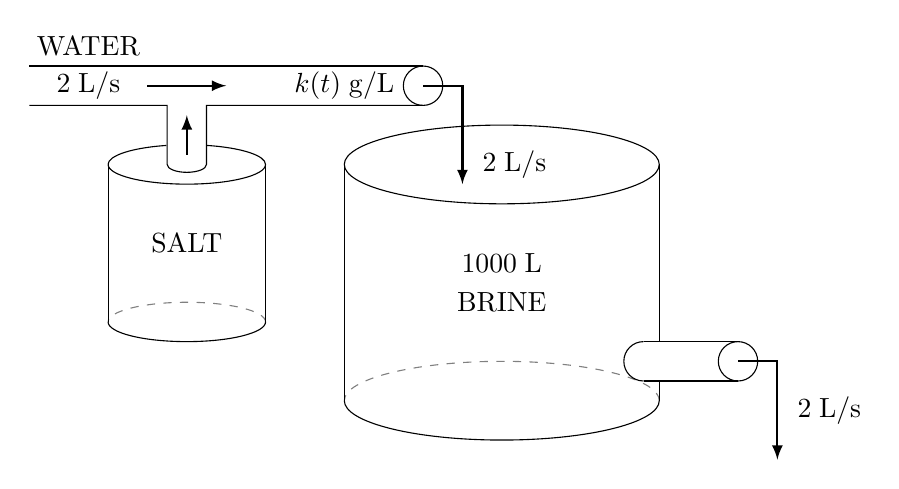
\begin{tikzpicture}

	% tank
	\draw[dashed,gray] (2,0) arc (0:180:2cm and 0.5cm);
	\draw (2,0) arc (0:-180:2cm and 0.5cm);
	\draw (0,3) ellipse (2cm and 0.5cm);
	\draw (-2,0) -- (-2,3);
	\draw (2,0) -- (2,0.25);
	\draw (2,0.75) -- (2,3);

	\draw (3,0.5) circle (0.25cm);
	\draw (1.8,0.75) -- (3,0.75);
	\draw (1.8,0.25) -- (3,0.25);
	\draw (1.8,0.75) arc (90:270:0.25cm);
	\draw[-latex,thick]
	  (3,0.5)
	  -|
	  node[near end,xshift=0.66cm] {$2 \; \mathrm{L}/\mathrm{s}$}
	  (3.5,-0.75);

	\draw (-1,4) circle (0.25cm);
	% \draw (-3.25,4.25) -- (-1,4.25);
	% \draw (-3.25,3.75) -- (-1,3.75);
	\draw[-latex,thick]
	  (-1,4)
	  -|
	  node[at end,xshift=0.66cm,yshift=0.25cm] {$2 \; \mathrm{L}/\mathrm{s}$}
	  (-0.5,2.75);

	\node at (-2,4) {$k(t) \; \mathrm{g}/\mathrm{L}$};

	\node at (0,1.75) {$1000 \; \mathrm{L}$};
	\node at (0,1.25) {BRINE};

	% salt source
	\draw[dashed,gray] (-3,1) arc (0:180:1cm and 0.25cm);
	\draw (-3,1) arc (0:-180:1cm and 0.25cm);
	\draw (-3,3) arc (0:75:1cm and 0.25cm);
	\draw (-5,3) arc (180:105:1cm and 0.25cm);
	\draw (-3,3) arc (0:-180:1cm and 0.25cm);
	\draw (-5,1) -- (-5,3);
	\draw (-3,1) -- (-3,3);

	\draw (-6,4.25) -- (-1,4.25);
	\draw
		(-6,3.75) -- (-4.25,3.75) -- (-4.25,3)
		arc (-180:0:0.25cm and 0.1cm)
		-- (-3.75,3.75) -- (-1,3.75);

	\node at (-4,2) {SALT};

	\node at (-5.25,4) {$2 \; \mathrm{L}/\mathrm{s}$};
	\node at (-5.25,4.5) {WATER};
	\draw[-latex,thick] (-4.5,4) -- (-3.5,4);
	\draw[-latex,thick] (-4,3.125) -- (-4,3.625);

\end{tikzpicture}
